\documentclass[b5paper]{article}

%% Language and font encodings
\usepackage[english]{babel}
\usepackage[utf8x]{inputenc}
\usepackage[T1]{fontenc}
\usepackage[parfill]{parskip}

%% Sets page size and margins
\usepackage[b5paper,top=3cm,bottom=2cm,left=3cm,right=3cm,marginparwidth=1.75cm]{geometry}

% add subfigures
\usepackage{subcaption}

%% enable multiple citing at once
\usepackage{cite}
%% enable url in citing
\usepackage{url}

%% Useful packages
\usepackage{amsmath}
\usepackage{graphicx}
%\usepackage[colorinlistoftodos]{todonotes}
\usepackage[colorlinks=true, allcolors=blue]{hyperref}
\usepackage{titling}
\usepackage[export]{adjustbox}
\usepackage{fancyhdr}
\usepackage{hyperref}

% packages for road map
% https://tex.stackexchange.com/questions/196794/how-can-you-create-a-vertical-timeline
\usepackage{array, booktabs}
\usepackage[x11names,table]{xcolor}
\usepackage{caption}

% define CrypkoPurple used in icon: 0xB0B1D5
\definecolor{CrypkoPurple}{RGB}{176,177,213}
% darker purple for caption text of table
\DeclareCaptionFont{blue}{\color{CrypkoPurple!70!black}}
\newcommand{\RoadMapStyle}{\color{CrypkoPurple}\makebox[0pt]{\textbullet}\hskip-0.5pt\vrule width 1pt\hspace{\labelsep}}


%% cross-ref list
%% https://tex.stackexchange.com/questions/1230/reference-name-of-description-list-item-in-latex
\makeatletter
\let\orgdescriptionlabel\descriptionlabel
\renewcommand*{\descriptionlabel}[1]{%
  \let\orglabel\label
  \let\label\@gobble
  \phantomsection
  \edef\@currentlabel{#1}%
  %\edef\@currentlabelname{#1}%
  \let\label\orglabel
  \orgdescriptionlabel{#1}%
}
\makeatother

%% Add logo
% https://www.overleaf.com/15705485shkbqqyzyxqs#/59720786/
% enable fancy page style on every page (the first page is excluded somehow?)
\pagestyle{fancy}
% first, clear default header
% https://texblog.org/2007/11/07/headerfooter-in-latex-with-fancyhdr/
\fancyhead{}  
% do not remove rule line
% \renewcommand{\headrulewidth}{0pt}
% \renewcommand{\footrulewidth}{0pt}
\setlength\headheight{50.0pt}
\addtolength{\textheight}{-50.0pt}
% add logo aligned to the left
\lhead{\adjincludegraphics[height=55pt, trim={0 {.2\height} 0 {.2\height}},clip]{logo-05.png}}


%% Add image above the title
\pretitle{
  \begin{center}
  \LARGE
  %  trim={<left> <lower> <right> <upper>}
  % width=\textwidth,
  \adjincludegraphics[width=\textwidth,trim={0 {0.05 \height} 0 {.35\height}},clip]{introduction2.png}\\
}
% \posttitle{\end{center}}
% The line below removes space directly below the date,
% which here is also directly above the abstract
% https://tex.stackexchange.com/questions/394041/reduce-the-top-margin-of-the-abstract
\postdate{\end{center}\vspace*{0em}}

% better use white paper?
% https://www.hipb2b.com/blog/white-paper-or-whitepaper-the-final-word-or-two/
\title{Crypko White Paper \\
  \large Cryptocollectible Game Empowered by Generative Adversarial Networks\\
  \rightline{\small ver 0.9.0 for comike}
}
\author{}
\date{}

\begin{document}

\maketitle
\newpage

\begin{abstract}

We propose a new type of online trading card game (TCG) where cards are cryptocollectibles whose images are created by generative adversarial networks (GAN), an promising AI technique. 
It has several advantages over conventional online TCG:
\begin{enumerate}
\item Each card, drawn by AI, is unique in appearance.
\item Users can freely trade cards with effectively real money in the market.
\item Users have true ownership of their cards, including their copyrights. % thanks to censorship-resistant Ethereum.
\item The same set of cards can naturally extend to various games. % thanks to borderless and permissionless Etherereum
\end{enumerate}

We are developing Crypko as an example of GAN-empowered cryptocollectible games with cards of anime characters.
The same idea can be applied to other domains of images as well.

\end{abstract}

% no page style on first page
\thispagestyle{empty}

\newpage

\section{Introduction}

The year of 2018 sees artificial intelligence and blockchain attracting wide attention.
However, most general people feel it hard to understand or only partially understand either technology. Researchers and mass media provide beautiful blueprints, but people do not know the current stage of development in AI and blockchain, what they two can do, and how they are changing our lives. 

On the other hand, these two technologies developed mostly independently. Few works could cross the boundary and combine their advantages, let alone involve general customers. 

To address this gap, we propose Crypko, a cryptocollectible game empowered by generative adversarial networks (GAN) that combined advantages of AI and blockchain. To be specific, in Crypko,

\begin{itemize}
\item Blockchain and smart contract ensure the value and ownership of digital property.
\item GAN generates various anime character avatars that worth appreciating and collecting.
\item By exploiting the property of generative networks, a smart contract can define and execute the fusion of two generated images, with which the game becomes more playable since the outcome of fusing is \emph{both} trackable and unpredictable. 
\end{itemize}

\subsection{Cryptocollectible game}

On November 28, 2017, the debut of CryptoKitties\cite{cryptokitties} brought cryptocollectible game, a new type of decentralized application (DAPP), under the spotlight, after which many companies and teams proposed their cryptocollectible games\cite{cryptomons,cryptocountries,cryptopets,cryptoarts,cryptolandmarks,cryptofighters,etheremon,etherwaifu}. As the subject of this type of games, cryptocollectibles are digital collectible whose ownership and uniqueness are secured by blockchain, and are referred to as breedable when two of them are capable of giving birth to a new one.

Cryptocollectible game has several advantages over conventional online TCG:
\begin{enumerate}
\item Users can freely trade cards with effectively real money in the market.
\item Users have true ownership (in terms of in-game property, not in real world) of their cards, thanks to censorship-resistance of Ethereum.
\item The same set of cards can naturally extend to various games, thanks to borderless and permissionless properties of Etherereum.
\end{enumerate}

\subsubsection{The brand new type of DAPP pioneered by CryptoKitties}

CryptoKitties pioneers a new type of DAPP in proposing following ideas. 
We highly appreciate these innovations and would like to carry over these ideas of CryptoKitties through our Crypko.

\begin{enumerate}
\item Publishing a DAPP in an existing blockchain can be both profitable and simple, which encourages practical blockchain applications. As a consequence, Initial Coin Offering (ICO) no longer serves as the only funding model for blockchain project.
\item Under the regulation of ERC-721, namely the Non-Fungible Token (NFT) Standard, cryptocollectibles are immutable and not fungible, thereby providing a foundation of its digital scarcity and value.
\item Through gamification, anyone can experience the convenience and revolution brought to us by blockchain without caring complex technical details.
\item The game operates on a sustainable revenue model by receiving a birth fee, transaction fee and from Generation 0 cryptocollectibles sales.
\item Two existing NFTs can breed a new NFT to ensure both randomness and user controllability of the creation process.
\end{enumerate}


\subsubsection{New cryptocollectible games following CryptoKitties}
After releasing of CryptoKitties, there have been several attempts to design cryptocollectible game by extending CryptoKitties, 
mostly by introducing battle mechanism between NFTs\cite{cryptofighters,fishbank,cryptomons,etheremon} based on smart contracts. 
Although such mechanism is a good point in designing gameplay,
the current speed of execution of smart contracts on blockchain is preventing effective implementation of any turn-based or real-time Ethereum games.

Other cryptocollectible games extend the object of NFT from cat to other animal\cite{cryptopets,etheremon}, or even beyond living things to territories\cite{cryptocountries}, places of interest\cite{cryptolandmarks} or paintings\cite{cryptoarts}. 
Nevertheless, those game typically do not enable reproduction, 
so users can no longer breed their own NFTs.

\subsection{Limitations of state-of-the-art cryptocollectible games}

Despite the progress, existing cryptocollectible games still leave much room for improvement to address following problems:

\begin{description}
\item [Problem 1\label{problem:1}] A cryptocollectible is composed of several mutually independent parts. For breedable cryptocollectibles, the generic heredity is discontinuous and lacks coherence since parts of different categories are mutually independent.
\item [Problem 2\label{problem:2}] Cryptocollectibles are not diverse in appearance. In a typical cryptocollectible game, there are only hundreds of types of parts, the combination of which may easily bore the users.
\item [Problem 3\label{problem:3}] The rarity of attributes defined by the game provider determines the value of a cryptocollectible. However, in reality, the value of a collectible is determined by its natural rarity.
\end{description}

\subsubsection{Inheritance lacks continuity, and attributes lacks diversity}

Placing an NFT in auction realizes its exchange value. 
On top of that, breeding, as the only way to create new NFTs from existing NFTs, 
serves as a significant element of a cryptocollectible game for sustainable revenue and customer stickiness.

Referring to real-world collectibles, designing an Ethereum game of breedable cryptocollectibles should also deal with the continuity of inheritance to an NFT from its parents. 
Breeding should show heredity (at least to a certain degree), namely the passing on of physical characteristics from parents to their child, as in the real world.

Existing approaches can be roughly categorized into two kinds: 
(1) drawing the image of every NFT though the intensive use of labor, leveraging illustration experts for showing proper way of inheritance, and 
(2) breaking the inheritance to a child NFT into a composition of independent parts inherited from parent NFTs. 
Although the first kind of approaches could produce an image with the best quality, its intensive labor of drawing individual images for every new-born NFTs prohibits its application in breedable cryptocollectibles.

As a more practical yet of-less-quality solution, the second kind of approaches is adapted by typical cryptocollectible games\cite{cryptokitties,etherwaifu,cryptofighters} which determine the new NFT's gene through recombination and mutation of the parents' genes, thus the combination of parts of the child. Although it avoids the intensive labor of drawing individual images by resorting to the combination of mutually independent attributes, the breeding of NFTs inevitably degenerates into "dress up game".

Furthermore, The vast number of combination of parts does not eliminate users' boredom, since the difference of NFTs only reflects on the difference of combination of parts, but not parts themselves. However, illustrators can draw only a limited number of parts --- in fact, a typical cryptocollectible is composed of less than ten types of parts, each of which has around ten variations. Thus the uniqueness of an NFT, despite combinatorially correct, is not visually intuitive.

In an attempt to circumvent such an issue, some game providers issue a limited number of copies of a type of special NFT drawn as a unity. However, these NFTs not only lose the continuity of heredity but also break the uniqueness of cryptocollectibles.

\subsubsection{Value = Artificial rarity = Sum of rarity of parts?}

In the auction house of a typical cryptocollectible game, the price of an NFT is determined by either the scarcity or the rarity of its parts, directly labeled by the game provider.

However, in a real-world auction house, a collectible is priced by its publicly perceived rarity. It is natural to apply the same logic to cryptocollectible games, but following issues remain:

\begin{itemize}
\item A collectible of physical existence is naturally rare. However, when a game provider determines the rarity of cryptocollectibles, it also controls the pricing rule, therefore compromising the decentralization of the game.
\item A person purchase a collectible because it matches his/her perception of beauty. However, when market values NFT that are rare (as specified by game providers) rather than aesthetically pleasing, NFTs cease to demonstrate their intrinsic value and beauty, degrading to bargaining chips. 
\end{itemize}

\subsubsection{Owning a cryptocollectible without owning its copyright?}

It is impossible to assign the copyright to the owner if an NFT is composed of parts, because copyright implies owner's rights over every parts of the image, but in reality they are shared by many other NFTs.

Since a user owns an NFT without owning its copyright, the ownership is completely restricted to blockchain: the owner can of course trade or breed their NFTs, but holds barely any other practical value.

\subsection{Generative Adversarial Networks}

Introduced by Ian Goodfellow et al. in 2014, Generative Adversarial Networks (GAN)\cite{goodfellow2014generative} are a class of deep learning algorithms that can train neural networks to generate highly authentic images. Subsequent works quickly and largely improve both the authenticity and the resolution of images generated by GAN models to a remarkable level\cite{radford2015unsupervised,karras2017progressive}, 
demonstrating their strong potential for applications to various application scenarios.

\subsubsection{MakeGirlsMoe - Create Anime Characters with A.I.!}

Prior to Crypko, we focused on the generation of anime avatars by GAN. In August 2017, we released \href{http://make.girls.moe/#/}{make.girls.moe, or MakeGirlsMoe}, a system for customizable generation of anime characters.

In MakeGirlsMoe (MGM), the GAN model trained on our cleaned anime dataset masters the generation of diverse, high-quality and customizable anime facial images. \emph{Amaryllis}, our first model, generates avatars of size $128 \times 128$ in a browser, after which \emph{Camellia}, our third model, push the resolution to $256 \times 256$ in December 2017.

The website attracts visitors from all over the world, mainly Japan, US, China, and Russia. By February 1, 2018, the total number of visits amounts to 1.5 million, peaking at 230 thousand in a single day.

MGM also receive recognition in academia. Having disclosed the website, we unveiled the technique of GAN behind MGM on arXiv\cite{jin2017towards}. In December, our paper is presented at \href{https://nips2017creativity.github.io/}{the Workshop on Machine Learning for Creativity and Design in NIPS 2017}.

\subsubsection{Impediment to practical applications of pure GAN}

The most straightforward practical GAN application, or a pure GAN application in this article, profits by providing image generation as a service. For example, pure GAN applications include retail of generated images, but not GAN assistant design.

As a free, highly reviewed service on GAN, MGM is not intended to be a revenue model. More generally, the same obstacle exists for almost any pure GAN application: generated images, however exquisite, can hardly possess enough exchange value. Since a generator is capable of producing an infinite number of possible images, abuse of a readily available generator will deprive its generated images of digital scarcity. Therefore, it is the advantage of GAN that impedes any practical application.

Two possible approaches are necessary to endow generated images with exchange value.

\begin{enumerate}
\item Preclude the abuse of generator, such as requiring payment for the service of generation.
\item Allow the right user to claim the ownership of a generated image to secure its digital scarcity.
\end{enumerate}

Approach 1 is intuitive, but without approach 2, a user can never be free of worries when, for example, sharing on a social media the generated images he or she has purchased. Nevertheless, approach 2 seems impossible, until the arrival of ERC-721. 

\section{The Product}

A Crypko is a cryptocollectible card of an anime character that a user can trade or fuse with another card into a new card.

Every Crypko is encoded into a code and a group of attributes, or collectively named as its representation. The representation determines a unique facial drawing of size $512 \times 512$. The group of attributes explicitly specifies some visual characteristics of a Crypko, while the code implicitly adjusts any other appearance and details.

The attributes of a Crypko reflect on its appearance to some extent. Different from a typical cryptocollectible game, two Crypkos can have distinct appearances even when they coincide in attributes.

A user can fuse two cards, the origins, into a new card, the derivative. The origins will not disappear but be on a limited cooldown after fusion, and the cooldown will take longer after each fusion. The result of fusion is not predictable, but the derivative should resemble its two origins to a certain degree. Besides a user's card, the user can also rent a card from another user for fusion.

A Crypko without origins is an Iteration 0 Crypko (or simply Iter 0 Crypko). 50 thousand Iter 0 Crypkos will enter the market automatically one every 15 minutes by auction. We will disclose at the beginning the representation of all Iter 0 Crypko.

In theory, a Crypko can fuse into infinite number new Crypkos, with the total population of Crypko and its growth in control: the cooldown takes longer when the Crypko has a higher iteration number or has been fused for more times; after we distribute all Iter 0 Crypkos, fusion is the only way to create a new Crypko.

Etymologically, Crypko is the composition of ``Crypto'' and ``ko'', which means a boy or a girl in Japanese.

\section{Advantages}

Crypko solves \ref{problem:1} - \ref{problem:3} using GAN, thereby exploring the potential of cryptocollectible games.

\subsection{Continuous fusion}

\begin{figure}[h]
  \centering
  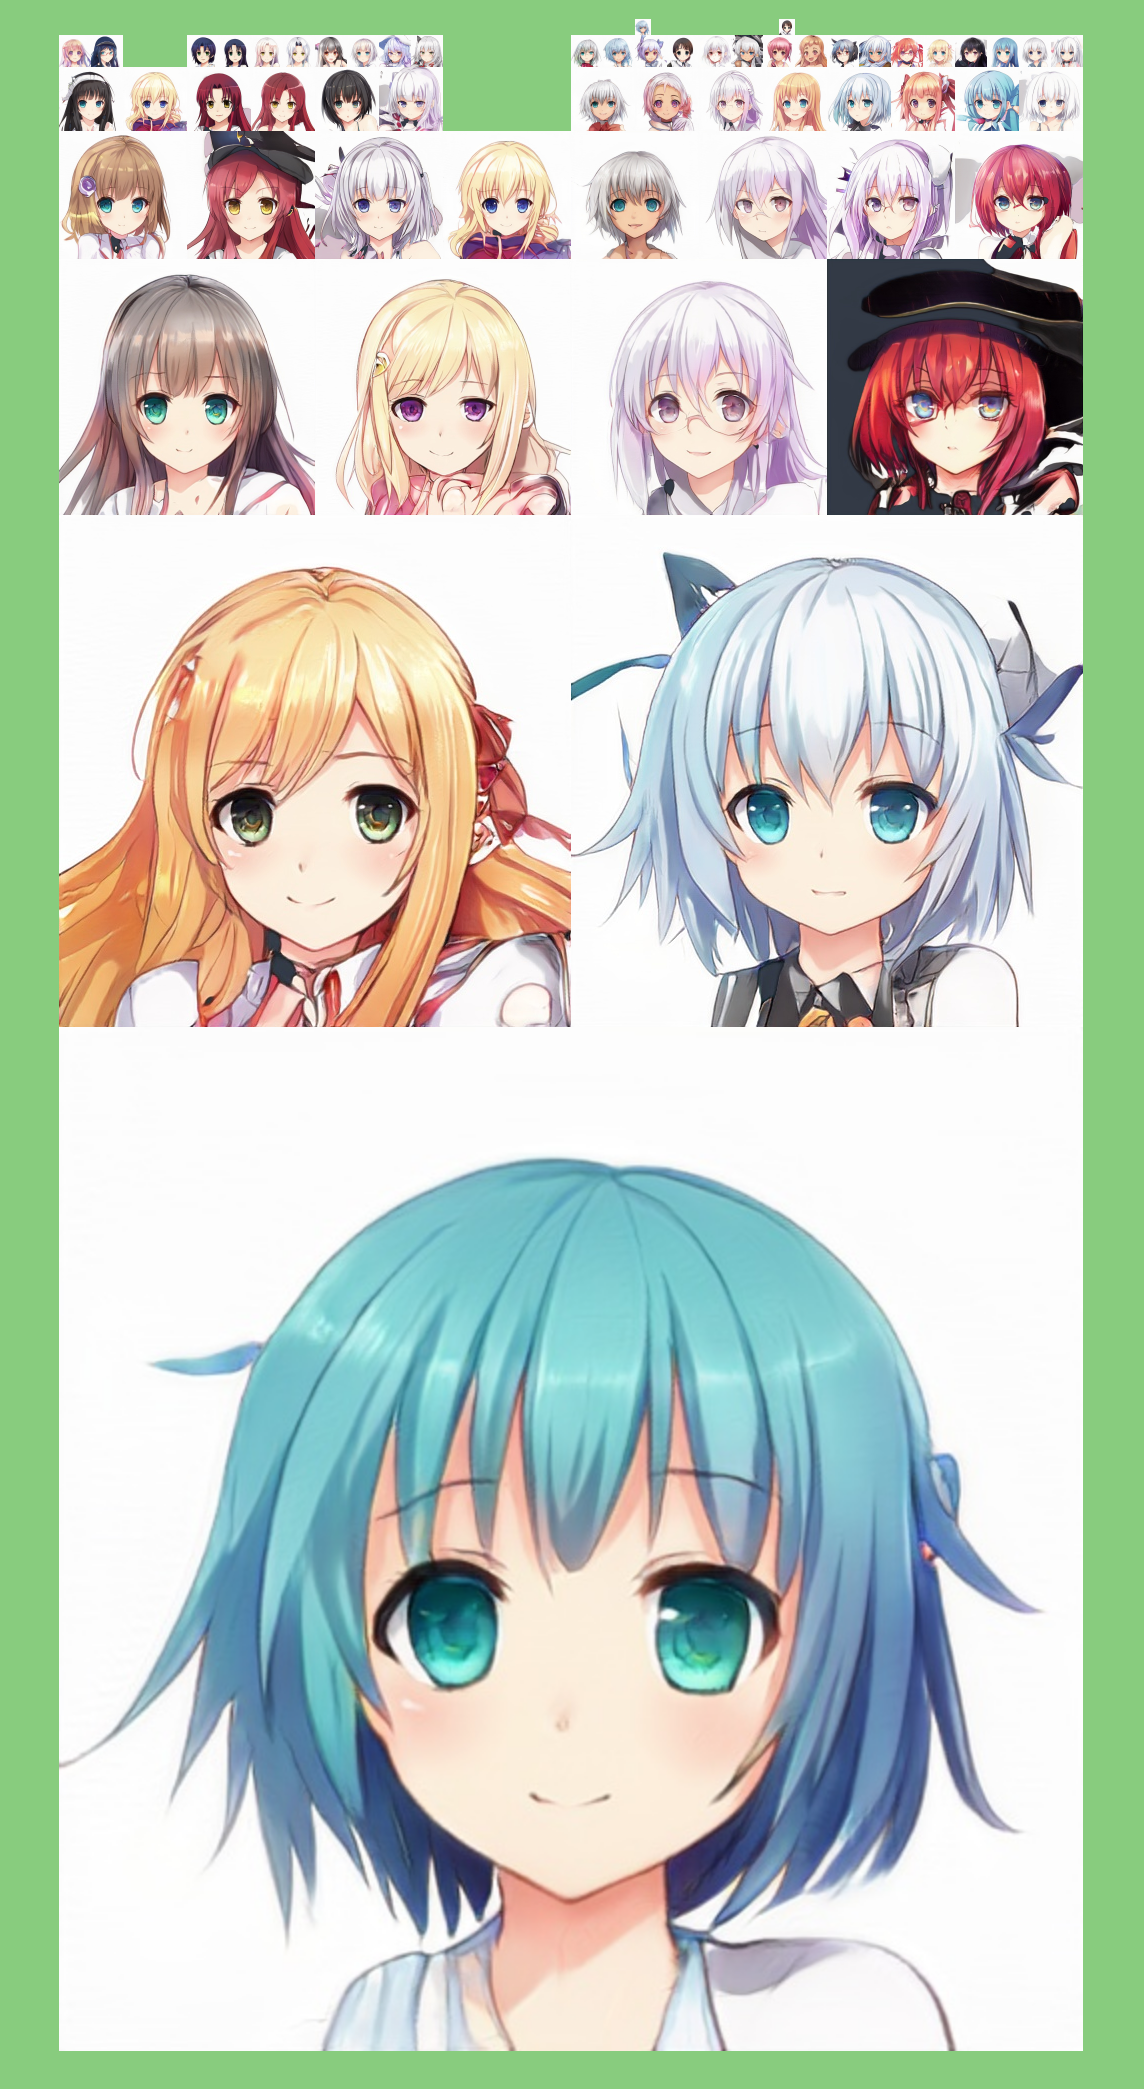
\includegraphics[width=0.55\textwidth]{703057_tree.png}
  \caption{Continuous fusion - origins tree}\label{origins_tree}
\end{figure}

The continuity of fusion is the property that the result of fusion does not duplicate almost any part of the materials of fusion, but is a coherent image as a whole representing a fine-grained coherent inheritance of materials.

In Crypko, fusion is based on vector arithmetic operations in the latent space of the generator\cite{radford2015unsupervised}. The generator takes a representation vector as input and outputs the corresponding image. Therefore, if we ``fuse'' the genes of two images appropriately, we get a new image that shares the characteristics of both images.

Consequently, we solve \ref{problem:1} and \ref{problem:2}. 
Our generator masters the principle of drawing, and understands the distinction between Crypkos after trained on anime characters dataset. 
As a result, fusion is no longer a simple re-combination of parts of two Crypkos but produces from thin air a new Crypko that shares the characteristics of both origins based on their codes.

Fusion introduces a little controllability to this game of randomness: if a user selects appealing Crypkos for fusion, the new Crypko will probably be appealing, too.

We believe the intuitiveness of continuous fusion and the diversity of derivatives will engage users' interest.


\subsection{Value = Appealingness}

Besides continuity, the use of coding that is then processed by a generator introduces a brand new pricing rule with the following two properties:

\subsubsection{Complexity of implicit representations}

The intention of setting up attributes of a Crypko is solely for the convenience of searching and filtering, but not for determining its value, so we refrain from any manipulation of the rarity of attributes.

In fact, as the implicit representation of the appearance of a Crypko, the code determines Crypko's exquisiteness and appealingness. Therefore, in Crypko, there is no outstanding attribute -- Crypko will not be more valued because its hair is blonde rather than black -- but only outstanding code. 

Since the mechanism of implicit representation is exactly the black box of deep learning, no one can decipher the meaning of its code with current technology.

\subsubsection{Integrity of code}

Since the code is indecipherable, any fragment of the code is meaningless, implying its integrity. Therefore, the fact that a Crypko is recognized as exquisite only prove its code, as a unity, but not any fragment of the code, is exquisite. Equivalently, the value of a Crypko reflects on its integrity, but not some of its parts. Therefore, we separate the value of Crypko as a cryptocollectible from its awkward and discrete labels.

Consequently, the pricing rule becomes subjective, since a user cannot evaluate a Crypko by its worthless attributes or unintelligible code. The independence of attributes and price rule out the possibility to calculate the price from data. Under the circumstances, a user can only trust on the attractiveness of Crypko for pricing.

And this is our expected cryptocollectible game mode: users subjectively evaluate the price of Crypko by their eye, and trade and fuse correspondingly.

Our game mode has benefits over other cryptocollectible games, namely:

\begin{enumerate}
    \item Significantly lower the barrier for the game. Imagine that in a real auction house or a typical cryptocollectible game, even if the user has created the account and deposited some cash, there is a psychological obstacle before trading: lacking understanding of pricing and experience in purchasing, the user might doubt that he or she can buy a worthwhile cryptocollectible. With the incomprehensible structure and parameters of a generator network and the randomness of fusion, Crypko does not grant a veteran a significant advantage over a novice.
    \item Having crashed the objectiveness of pricing, game provider cannot easily control the market anymore. In a typical cryptocollectible game, as long as the game provider decrease the frequency of a gene, the corresponding attribute becomes rarer, and hence more valuable. However, with a subjective pricing rule, everyone has their own taste, so the market only regards Crypkos adored by the majority of users as valuable.

\end{enumerate}

\subsection{Copyright belongs to the owner}

\begin{figure}[!h]
\begin{subfigure}{0.5\textwidth}
  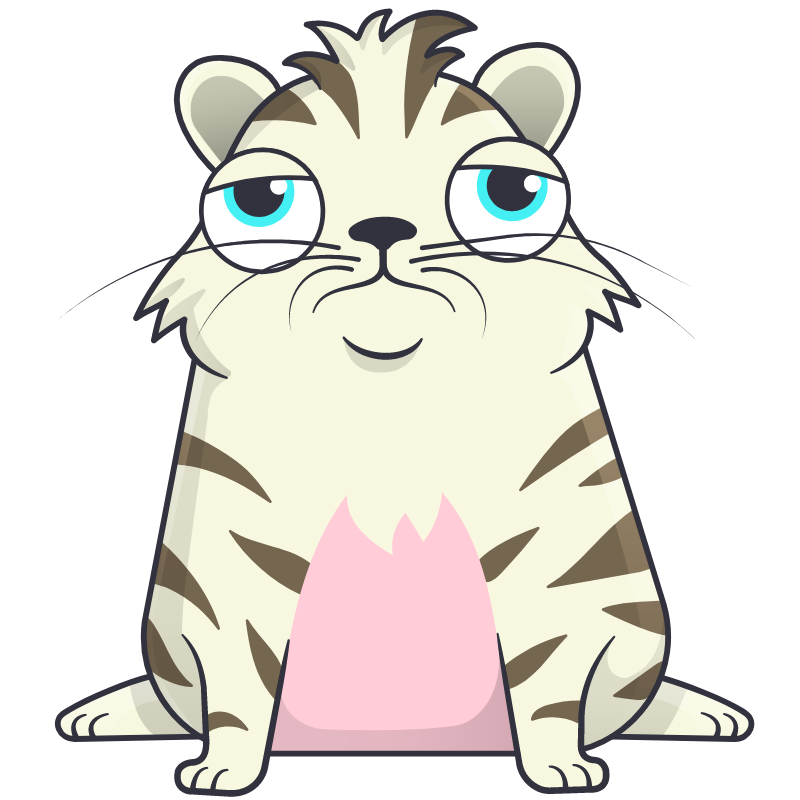
\includegraphics[width=\textwidth]{870796.png}
\end{subfigure}\hspace*{\fill}
\begin{subfigure}{0.5\textwidth}
  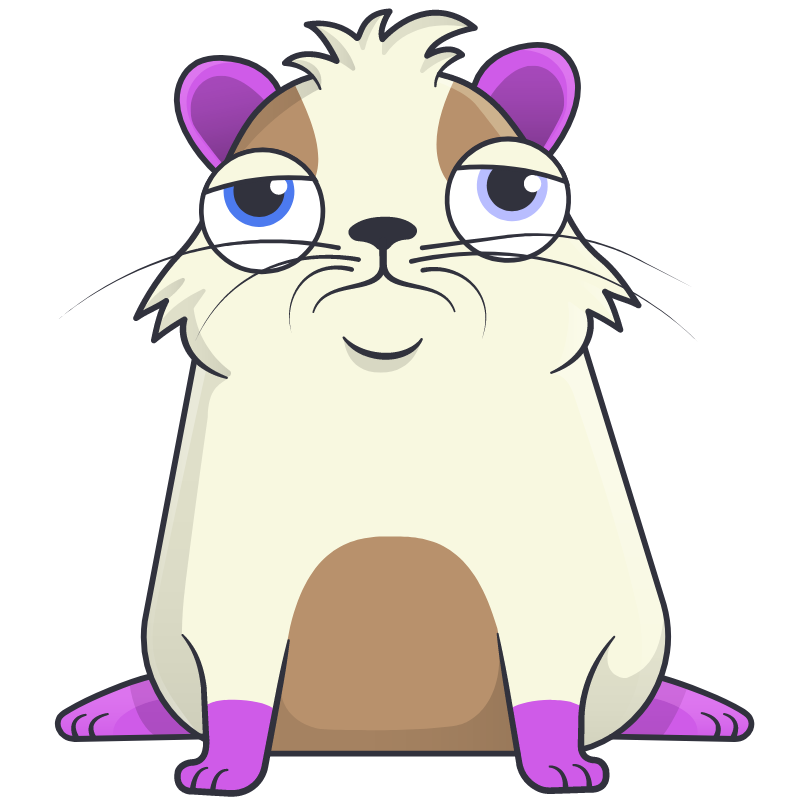
\includegraphics[width=\textwidth]{871240.png}
\end{subfigure}

\caption{
Traditional Cryptocollectible games cannot assign copyright of images to users, because collectibles with same attributes share the same image parts. Image source: CryptoKitties \cite{cryptokitties}.
}
\end{figure}

\begin{figure}[!h]
\begin{subfigure}{0.5\textwidth}
  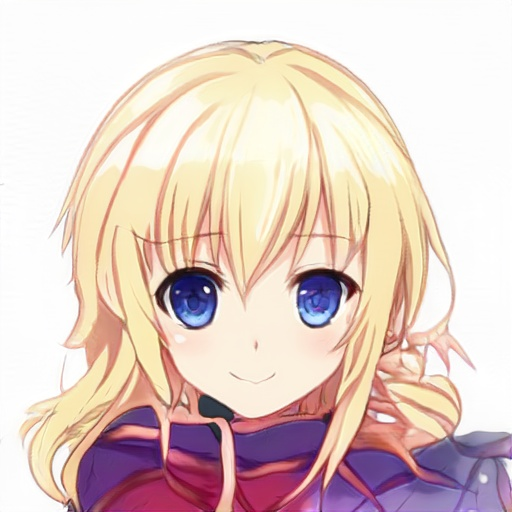
\includegraphics[width=\textwidth]{578.jpg}
\end{subfigure}\hspace*{\fill}
\begin{subfigure}{0.5\textwidth}
  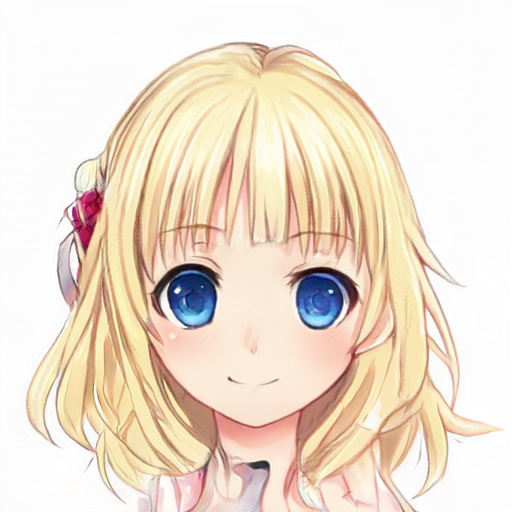
\includegraphics[width=\textwidth]{280706.jpg}
\end{subfigure}

\caption{
Crypko assigns copyright to users because even Crypkos with identical attributes does not share image parts.
}
\end{figure}


Since every Crypko is unique both as an entirety and in its parts, it is possible for us to design the game such that the copyright of a Crypko belongs to its current owner rather than us, the game provider.

In this way, the owner can use the image of his/her Crypko as it is for commercial usage, including usages as a character in his/her novels or RPG games. 

Furthermore, the owner can create derivative works of his/her Crypko for commercial usage.
Although there are countless derivative works based on copyright-protected anime works, such acts are in the legal grey areas. However, the owner of a Crypko can, without any dispute, create derivative works based on the Crypko.

Notice that if the owner decides to sell his/her Crypko later on, he/she will lose the copyright of the Crypko thereafter, as if he/she had sold the copyright of an artwork he/she created.

\section{Beta Test}

We have arranged an open beta of Crypko from 13th May to 5th August. 
The user interface is public at \href{http://crypko.ai}{ crypko.ai }. Visitors can access the market via any browser (desktop or smartphone) to view the Crypkos created by beta users.

During the beta test, a user was able to use \href{https://metamask.io/}{MetaMask plugin} in Chrome or Firefox, or a mobile wallet browser such as \href{https://trustwalletapp.com/}{Trust - Ethereum Wallet} or \href{http://www.buntoy.com/} {BUNTOY}, connect to Rinkeby test network and create an account, after which he or she could receive some Rinkeby ether from \href{https://www.rinkeby.io/#faucet}{Rinkeby faucet}, and try all features of Crypko including trading and fusion.

\section{Next Step}

We plan to reduce the friction of operation (Crypko v2) and introduce more gameplay into Crypko (Crypkosmos) soon.
We detail our proposed road map \footnote{Might subject to changes in schedule or content} in the follows.

\subsection{Crypko v2 - frictionless Crypko}

Cryptocollectible games, although having several advantages over traditional TCG games, 
are notorious for slow transaction speed and high transaction fee (or gas fee in Ethereum jargon). 
To address these issue, we plan to leverage Ethereum layer 2 scaling soluctions such as \cite{poon2017plasma} into the next version of Crypko, in order to make the transactions easier in terms of time and fee, 
and to enable further game play with higher real-time requirement.

\subsection{Crypkosmos - the world of Crypko}

The true ownership of a Crypko makes it possible to create a world of Crypkos (we would like to call it \emph{Crypkosmos}), which is inspired by \href{https://www.cryptokitties.co/kittyverse}{KittyVerse}. 

Every user owns his/her unique set of Crypkos, 
therefore when he/she plays games licensed with Crypko's images, 
it is natural that he/she should also own the same set of Crypkos in these licensed game. 
For example, if someone developed an idol management game using Crypko's images under the permission of Crypko team, then a user can play the game with his/her Crypkos joining idol activities.

In another word, we envision the funciton of Crypko as both a marketplace and a card mint, 
and derivative games can be built upon Crypko, together forming the Crypkosmos. 
We plan to provide the necessary API and instruction to encourage developers create online card games based on Crypko cards by 

Since selling a Crypko implies selling anything related to the Crypko in Crypkosmos, 
if users value these in-game achievements or rare items, 
the value of a Crypko will be influenced by their activities in the derivative games. 
For example, we should expect a higher price when a Crypko has high charisma points in a derivative idol management game and a high level or equipped with rare items in a derivative MMORPG.
We plan to provide support in form of trading mechanism to accommodate such case.

\begin{table}
\centering
\renewcommand\arraystretch{1.4}\arrayrulecolor{CrypkoPurple}
\captionsetup{singlelinecheck=false, font=blue, labelfont=sc, labelsep=quad, justification=centering}
\caption*{Road Map}\vskip -1.5ex
\begin{tabular}{@{\,}r <{\hskip 2pt} !{\RoadMapStyle} >{\raggedright\arraybackslash}p{7cm}}
\toprule
\addlinespace[1.5ex]
Dec 2017 & Crypko project started.\\
Jan 2018 & Prototype completed.\\
Feb 2018 & Generative model "Daisy" trained. \\
Apr 2018 & Open beta pre-registration began.\\
May 2018 & Open beta started.\\
Summer 2018& Open beta ended.\\
& Popularity poll of beta Crypkos.\\
Autumn 2018 & Crypko official release.\\
 & Crypkosmos project start.\\
 & Crypko v2 project start.\\
 Winter 2018 & Crypko v2 closed beta.\\
 & Crypkosmos API documentation.\\
 2019 & Crypko v2 official release.\\
 & Crypkosmos extends to Crypko v2.\\
 
\end{tabular}
\end{table}

\section{Conclusion}

Given GAN as a promising technique for image generation, we expect Crypko go beyond being an yet-another new member of cryptocollectible games. 
We want to inspire the market of homogeneous cryptocollectible games with more games where a collectible has inner value and the game is both fun and rational.

On the other hand, since ERC-721 endows digital properties with value, 
we expect that after Crypko is deployed on Ethereum, 
there will be more deep learning developers willing to turn their generative models such as GAN~\cite{goodfellow2014generative}, VAE~\cite{kingma2013auto} or LSTM~\cite{hochreiter1997long} 
into a practical blockchain game demonstrating AI's value in creation. 
Meanwhile, we believe in the survival of the fittest tokens, which will, in turn, encourage the development of generative models.

Furthermore, by assigning the publicly verifiable copyright of a Crypko to its owner, we believe that Crypko can provide inspiration for creation of derivative works.

To make the game play more interesting, we are actively working on Crypko v2 and Crypkosmos, reducing the friction of operation and introducing more game play into Crypko.

We wish that the high-quality generative model of Crypko and the intuitive evaluation standard will attract more people to the game of cryptocollectible. We do not know how public will react towards Crypko, but we believe it proves the combination blockchain and AI can be simultaneously practical, meaningful, and fun.

We believe in the potential of blockchain, and the significance of cryptocollectibles.
Rare collectibles are valuable, but we genuinely believe that we should not stick price labels to cryptocollectibles according to artificial rarity. We treasure a cryptocollectible, because of its breathtaking beauty, and its manifold moe.

\vspace{5mm}

\begin{flushright}
 The Crypko Team
\end{flushright}

\bibliographystyle{plain}
\bibliography{bibliography}

\end{document}


